
Obbiettivo di questo primo capitolo è presentare gli ambiti dell'analisi di traiettorie toccati da questa tesi.
Saranno presentati due approcci: in primo luogo verrà trattato il clustering, successivamente il frequent itemset mining.
Per ciascuno di questi due ambiti verranno esposti le principali caratteristiche e le applicazioni nella ricerca di pattern di movimento.

\section{Dati di traiettoria}\label{sec:trajectorydata}
Negli ultimi anni, la grande presenza di dipositivi in grado di catturare la posizione di un oggetto nel
tempo e le sue variazioni hanno prodotto enormi quantità di dati.
L'analisi di questi dati, resa possibile dalle moderne tecnologie Big Data, apre molteplici possibilità, come
ad esempio la ricerca dei flussi di traffico all'interno di un terriorio cittadino, oppure l'individuazione
dei luoghi più visitati da una certa categoria di utenti, o ancora il riconoscimento di gruppi di oggetti che si
muovono assieme all'interno di un certo spazio e tempo.
Dato il grande numero di potenziali fonti per i dati, è necessario ricondurre questi ultimi a una formulazione comune
così da poter sfruttare al meglio le loro potenzialità espressive.
La rappresentazione più basilare consiste nel considerare una traiettoria come l'insieme delle posizioni
spaziali dei punti che la compongono associando a ciascuno l'istante temporale in cui è stato registrato.
Questa formulazione prende il nome di traiettoria grezza (\textit{raw trajectory}), vedi~\cref{fig:chap-1:trajectory}
Andando a formalizzare quanto detto sopra:

\begin{figure}
  \centering
  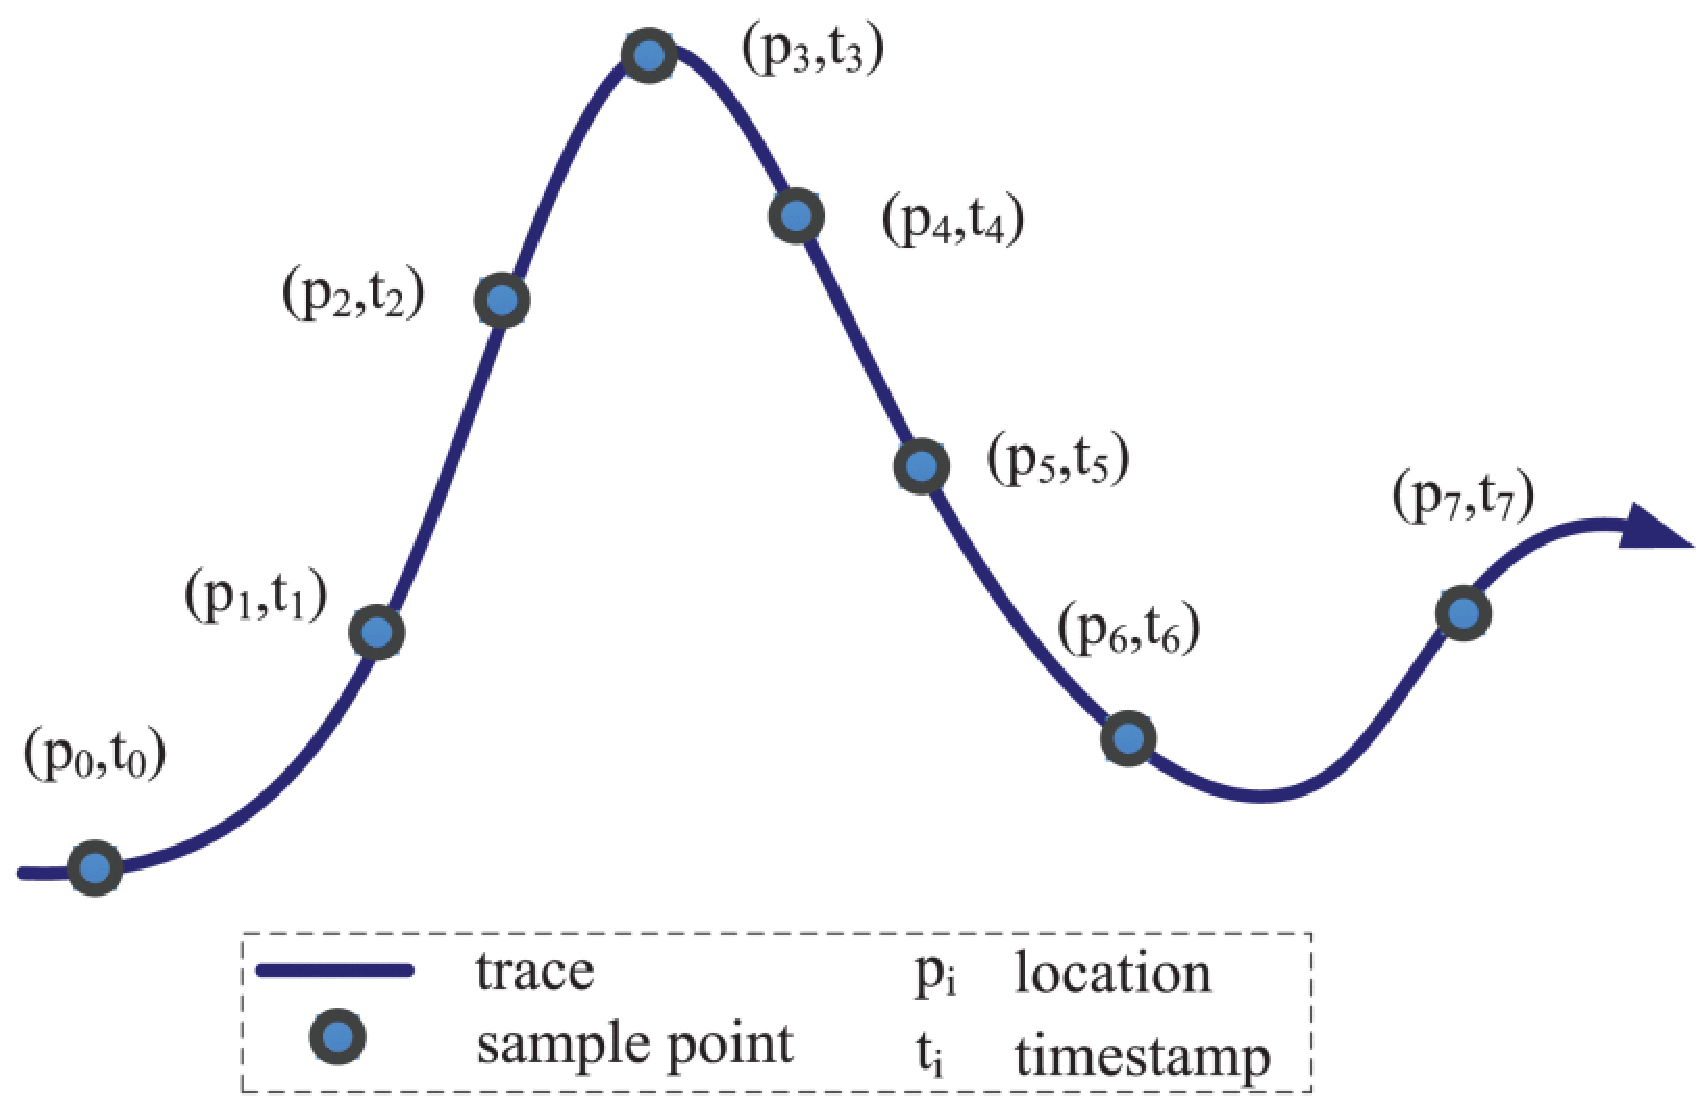
\includegraphics[scale=.5]{/sec-1/trajectory.pdf}
  \caption{Esempio di traiettoria,Fonte:\url{https://www.semanticscholar.org/paper/A-Survey-on-Trajectory-Data-Mining\%3A-Techniques-and-Feng-Zhu/a32f521442a540a6d1420526eaa68b3cab6b1d0d}}%
  \label{fig:chap-1:trajectory}
\end{figure}

\begin{definition}[Traiettoria]

  Si definisce una traiettoria grezza, o \textit{raw trajectory}, una sequenza temporale di punti \({p_{t}, p_{t'},\ldots, p_{t''}}\)
  tale che ogni punto \(p_{t}\) è composto da una coppia di coordinate spaziali \((latitude, longitude)\) e un tempo~\(t\).

\end{definition}

Questa basilare e semplice modalità di espressione può essere successivamente complicata, ad esempio adottando
una scala unica tra le diverse traiettorie per lo spazio e una per il tempo, oppure aggiungendo ulteriori informazioni, come ad esempio la direzione o attributi
dell'oggetto che la genera.

Per aumentare l'espressività della singola traiettoria, può essere utile definire il concetto di sotto-traiettoria, o \textit{subtrajectory}.
Intuitivamente una sotto-traiettoria non è altro che un segmento di una traiettoria relativo a un certo sottoinsieme dello spaziotempo coperto da quest'ultima.

\begin{definition}[Sottotraiettoria]

  Date due traiettorie \(TR\textsubscript{i}, TR\textsubscript{j}\) si definisce  \(TR\textsubscript{i}\) sottotraiettoria di \(TR\textsubscript{j}\) se \(\forall p_{t\textsubscript{i}} \in TR\textsubscript{i}, p_{t\textsubscript{i}} \in TR\textsubscript{j}\).

\end{definition}

Una volta definito che cos'è un dato di traiettoria, occorre mettere in chiaro che cosa distingue una traiettoria da un'altra.
Prendendo ad esempio il problema del clustering, sarebbe sbagliato tentare di applicare le stesse metriche di similarità anche ai dati di traiettoria
poiché gli oggetti in movimento producono spesso dati ad alta dimensionalità e con particolari correlazioni tra le dimensioni.
Il problema risulta quindi decisamente articolato: uno buona metrica di similarità deve tenere conto non solo dei singoli punti, ma anche della
traiettoria nella sua interezza, considerando anche la diversa lunghezza tra i due soggetti del confronto.
In letteratura sono presenti diversi metriche che possono essere impiegate nel confronto tra traiettorie:

\begin{itemize}

  \item \textbf{Distanza Euclidea.}
  La più semplice tra tutte le misure di stanza presentate, grazie alla sua complessità lineare permette di gestire dati ad alta dimensionalità.
  Date due traiettorie  \(T\textsubscript{i}\) e  \(T\textsubscript{j}\) di lunghezza \(n\) e dimensioni \(p\), la loro distanza euclidea si definisce come:

  \begin{equation}
    {D_E(T_{i}, T_{j}) = { {\frac{1}{n} } \sum_{k=1}^{n} {\sqrt{\sum_{m=1}^{p}{(a_{k}^{m} - b_{k}^{m})}^2}}}}
  \end{equation}

  La metrica tuttavia non è esente da difetti: è molto sensibile al rumore e richiede che le traiettorie siano uguali per numero di punti
  e dimensioni, inoltre anche l'intervallo di campionamento temporale deve coincidere. Questi limiti sono abbastanza difficili da
  aggirare quando si processa un dataset reale.

  Per superare questi problemi, sono disponibili diverse varianti della distanza euclidea: una su tutte è la \textit{Principal Component Analysis Plus Euclidean Distance} (PCA + distance)~\cite{zhang2006comparison}.
  Questa tecnica prima riduce le dimensioni spaziali ad una sola, successivamente esegue un'analisi PCA per convertire ogni traiettoria in
  \textit{k} coefficenti; a questo punto viene calcolata la distanza euclidea considerando i valori dei coefficenti individuati dall'analisi.
  Questa variazione mantiene gli stessi punti di forza della versione base della metrica, in più consente una maggior resistenza al rumore.



  \item \textbf{Distanza di Hausdorff.}
  La distanza di Hausdorff~\cite{chen2011clustering} misura quanto due traiettorie sono distanti l'una dall'altra.
  Date due traiettorie, per ogni punto di una viene calcolato il più vicino punto dell'altra e la distanza tra i due, il valore della distanza di Hausdorff
  corrisponde alla massima distanza calcolata nel passo precedente.~\cref{def:Hausdorff}
  \begin{equation} \label{def:Hausdorff}
    {D_{Hausdorff}(T_{i}, T_{j}) = \max{(h(T_{i}, T_{j}), h(T_{j}, T_{i}))}}~where~{h(T_{i}, T_{j}) = \max_{a \in T_{i}}{(\min_{b \in T_{j}}{(dist(a,b))})}}
  \end{equation}

  Nella formula \(h\) rappresenta la distanza di Hausdorff diretta, mentre \(d\) la distanza euclidea tra due punti.
  Il calcolo di entrambe le distanze dirette permette di gestire traiettorie con numero di punti differente tra loro.
  Questa metrica risulta robusta rispetto all'influenza causata da particolari distribuzioni di punti, ma allo stesso tempo è sensibile
  al rumore. Dalla formula~\cref{def:Hausdorff} è possibile definire la complessità computazionale della metrivca come \(O(m*n)\).


  \item \textbf{Distanza LCSS.}
  Longest Common Sub Sequence~\cite{rick2000efficient} affronta il problema con un approccio diverso: invece che calcolare la distanza fra i punti tra le due traiettorie, computa la
  più lunga sotto-sequenza.
  La lunghezza di quest'ultima determina la vicinanza,: più il valore è alto più le due traiettorie sono vicine.
  Essendo impossibile una coincidenza assoluta dei punti tra due traiettorie sono definite due soglie, \(\epsilon \) e \( \sigma \) che rispettivamente
  modellano la tolleranza rispetton all'asse x e y.
  LCSS può essere calcolata in modo ricorsivo, il suo tempo di computazione coincide con la diatnza di Hausdorff, inoltre consente una certa tolleranza rispetto
  alle deviazioni nei dati, ciò consente una buona efficenza nei dataset reali. Il maggior limite della metrica sta nella definizione dei parametri
  \(\epsilon \) e \( \sigma \) in problemi complessi.

  \item \textbf{Distnza DTW.}
  Dynamic time warping (DWT)~\cite{chen2005robust} pone il focus sulla dimensione temporale rispetto a quelle spaziali, come accadeva nelle metriche precedenti.
  Lo scopo è trovare l'allineamento ottimo tra due traiettorie dati certi vincoli.
  DWT resiste bene alle differenti lunghezze tra traiettorie: obbiettivo della misura è infatti ricercare il percorso a cui assimilare le traiettorie che abbia il minor coeficcente di distorsione,
  calcolato sulle trasformazioni subite dalle traiettorie.
  DWT assicura il rispetto dell'ordine tra i punti delle traiettorie, inoltre introducendo un principio di scaling locale della dimensione temporale,
  riesce a gestire scale temporali differenti tra le traiettorie.
  Tuttavia richiede continuità all'interno dei punti, è sensibile al rumore e a sottotraiettorie molto distanti tra loro.
  La complessità di questa misura è \(O(m*n)\).


  \item \textbf{Distanza di Fréchet.}
  La metrica di Fréchet~\cite{khoshaein2013trajectory} considera in contemporanea sia la dimensione temporale
  che quella spaziale durante il calcolo della distanza.
  Date due traiettorie di uguale lunghezza \(n\), si calcola la distanza euclidea tra i punti aventi stessa posizione all'interno delle due traiettorie:
  il valore più alto corrisponde alla distanza di Fréchet.
  Qualora le due traiettorie divergano come dimensioni, si eseguirà questo calcolo su tutte le possibili sotto-traiettorie di lunghezza \(n\) generabili
  dalla traiettoria più lunga.
  La complessità della misura nel caso peggiore è \(O(m*n)\).
  La distanza di Fréchet considera la traiettoria nella sua continuità, per questo motivo è molto sensibile agli outlier.


\end{itemize}





\subsection{Definizione di traiettoria}\label{subsec:trajectory-definition}
Dato il grande numero di potenziali fonti per i dati, è necessario ricondurre questi ultimi a una formulazione comune
così da poter sfruttare al meglio le loro potenzialità espressive.
La rappresentazione più basilare consiste nel considerare una traiettoria come l'insieme delle posizioni
spaziali dei punti che la compongono associando a ciascuno l'istante temporale in cui è stato registrato.
Questa formulazione prende il nome di traiettoria grezza (\textit{raw trajectory}), vedi~\cref{fig:chap-1:trajectory}.
Andando a formalizzare quanto detto sopra:

\begin{figure}
  \centering
  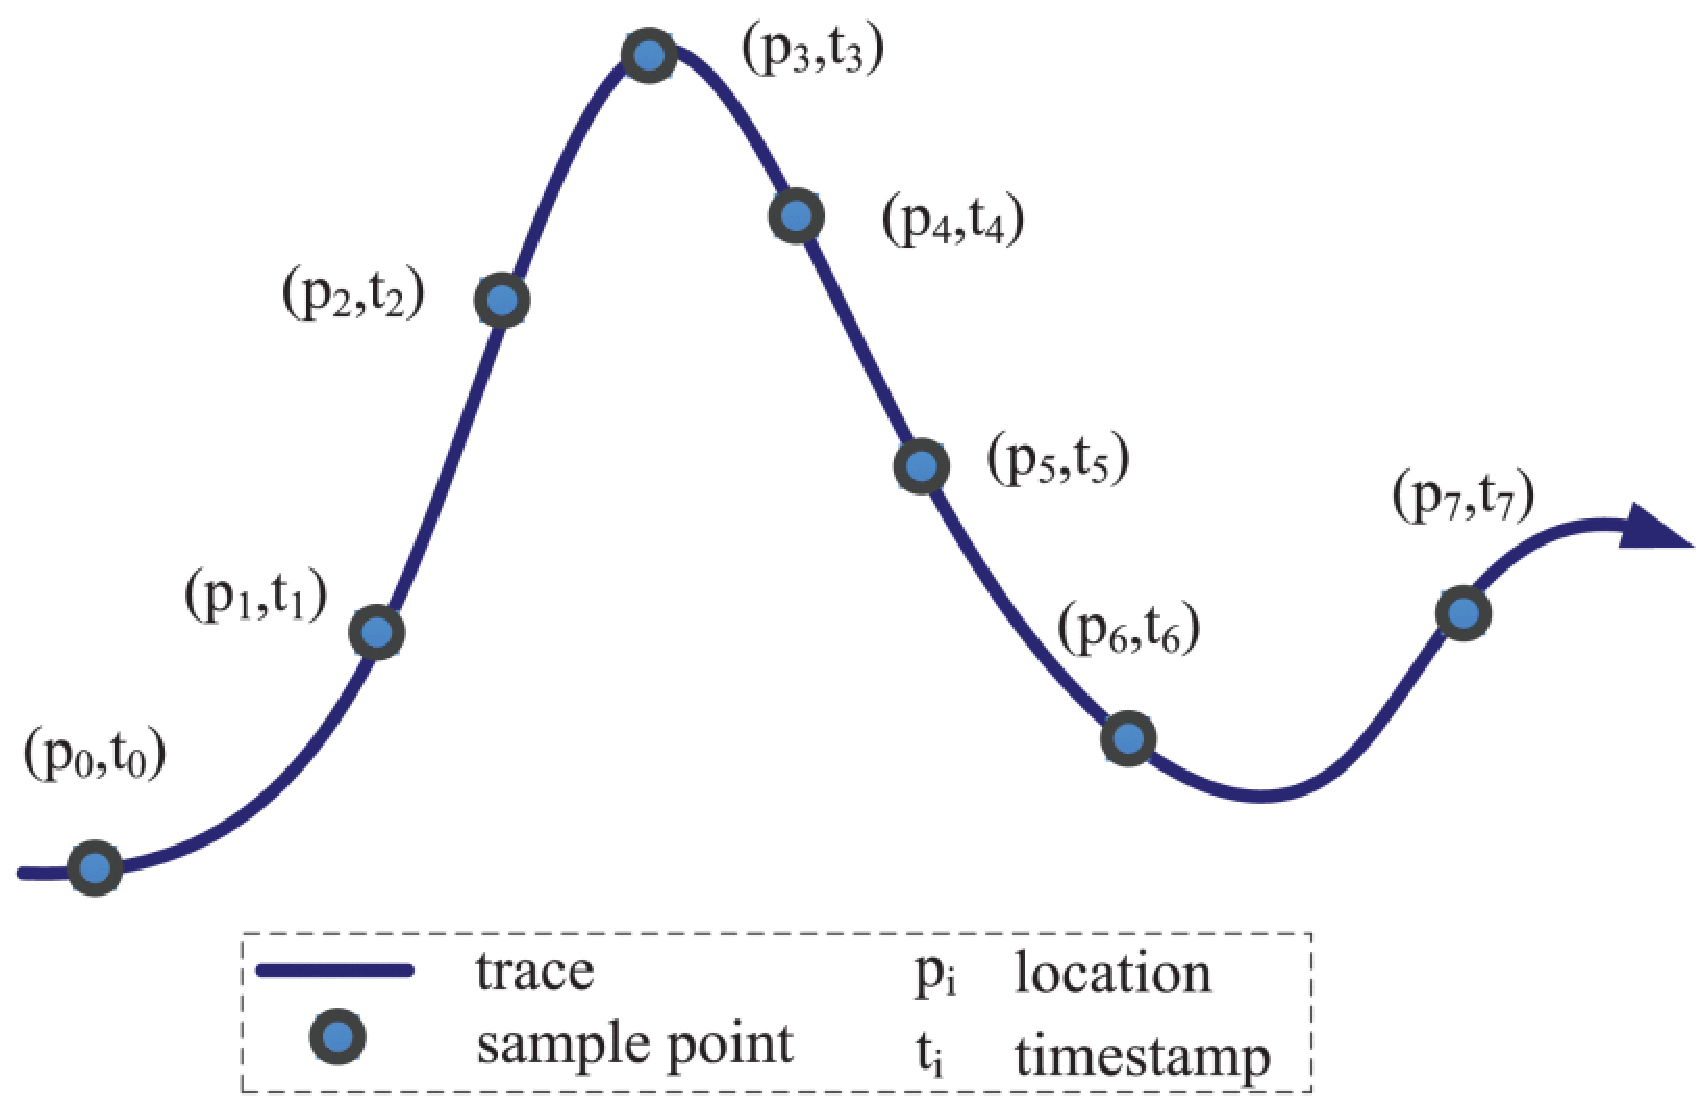
\includegraphics[scale=.7]{/sec-1/trajectory.pdf}
  \caption{Esempio di traiettoria, Fonte:~\cite{Feng2016ASO}}%
  \label{fig:chap-1:trajectory}
\end{figure}

\theoremstyle{definition}
\begin{definition}[Traiettoria]

  Si definisce una traiettoria grezza \(tr\) una sequenza temporale di punti \({p_{t}, p_{t'},\ldots, p_{t''}}\)
  tale che ogni punto \(p_{t}\) è composto da una coppia di coordinate spaziali \((latitude, longitude)\) e un tempo~\(t\).

\end{definition}

Tale formulazione può essere successivamente complicata, ad esempio adottando
una scala unica tra le diverse traiettorie per lo spazio e una per il tempo, oppure aggiungendo ulteriori informazioni, come ad esempio la direzione o altri attributi
dell'oggetto che la genera.

Per aumentare l'espressività della singola traiettoria, può essere utile definire il concetto di sotto-traiettoria, o \textit{subtrajectory}.
Intuitivamente una sotto-traiettoria non è altro che un segmento di una traiettoria relativo a un certo sottoinsieme dello spazio-tempo coperto da quest'ultima.

\begin{definition}[Sotto-traiettoria]

  Date due traiettorie \(tr\textsubscript{i}, tr\textsubscript{j}\) si definisce  \(tr\textsubscript{i}\) sotto-traiettoria di \(tr\textsubscript{j}\) se \(\forall p_{t\textsubscript{i}} \in tr\textsubscript{i}, p_{t\textsubscript{i}} \in tr\textsubscript{j}\).

\end{definition}

A queste definizioni va aggiunto il concetto di sistema di riferimento: si definisce un sistema di riferimento un insieme di
quanti completo e continuo all'interno di una regione spazio-temporale.
I sistemi di riferimento sono fondamentali nel determinare le dimensioni spazio-temporali dei punti delle varie traiettorie,
un esempio su tutti può essere una scala di riferimento espressa in coordinate polari.
Tuttavia è possibile definire anche sistemi di riferimento che utilizzano metriche diverse dalle coordinate sopracitate,
ottenendo così diversi effetti sulla rappresentazione dei dati.
Una traiettoria rappresentata secondo le coordinate di un certo sistema di riferimento si definisce \textit{trajectory abstraction} o astrazione di traiettoria:

\begin{definition}[Astrazione di traiettoria]

  Data una traiettoria grezza \(tr\) e un sistema di quanti spazio-temporali \( ST = \{q_{1},\ldots q_{n}\}\), un'astrazione di traiettoria è definibile come la sequenza di quanti  \( \{q_{i},\ldots q_{j}\}\) ottenuti esprimendo la traiettoria grezza \(tr\) sul sistema \(ST\)  .

\end{definition}



\subsection{Metriche di distanza}\label{sec:measure}
Una volta definito che cos'è un dato di traiettoria, occorre mettere in chiaro che cosa distingue una traiettoria da un'altra.
Per confrontare due traiettorie, sarebbe sbagliato applicare le metriche di similarità per dati a bassa dimensionalità,
poiché gli oggetti in movimento producono dati complessi e con particolari correlazioni tra le dimensioni.
Il problema risulta quindi decisamente articolato: una buona metrica di similarità deve tenere conto non solo dei singoli punti, ma anche della
traiettoria nella sua interezza.
A questo va sommata la diversa lunghezza tra i due soggetti del confronto.
In letteratura sono presenti diversi metriche che possono essere impiegate per confrontare due traiettorie:

  La prima tra tutte le misure è la distanza euclidea. Grazie alla sua complessità lineare permette di gestire dati ad alta dimensionalità.
  Date due traiettorie  \(tr\textsubscript{i}\) e  \(tr\textsubscript{j}\) di lunghezza \(n\) e dimensioni \(p\), la loro distanza euclidea si definisce come:

  \begin{equation}
    {dist(tr_{i}, tr_{j}) = { {\frac{1}{n} } \sum_{k=1}^{n} {\sqrt{\sum_{m=1}^{p}{(a_{k}^{m} - b_{k}^{m})}^2}}}}
  \end{equation}

  La metrica tuttavia non è esente da difetti: è molto sensibile al rumore e richiede che le traiettorie siano uguali per numero di punti
  e dimensioni, inoltre anche l'intervallo di campionamento temporale deve coincidere.
  Questi limiti sono abbastanza difficili da aggirare quando si processa un dataset reale.

  Per superare questi problemi, sono disponibili diverse varianti della distanza euclidea: una su tutte è la \textit{Principal Component Analysis Plus Euclidean Distance} (PCA + distance)~\cite{zhang2006comparison}.
  Questa tecnica prima riduce le dimensioni spaziali ad una sola, successivamente esegue un'analisi PCA per convertire ogni traiettoria in
  \textit{k} coefficienti; a questo punto viene calcolata la distanza euclidea tra le traiettorie così trasformate.
  L'~\cref{def:PCA} mostra la formula per il calcolo della distanza PCA + distance: \(a_{k}^{c}\) e \(b_{k}^{c}\) rappresentano i
  \(k\) coefficienti nello spazio bidimensionale delle traiettorie \(tr_{i}\text{,}tr_{j}\). 
  \begin{equation} \label{def:PCA}
    {dist(tr_{i}, tr_{j}) = {\sqrt{\sum_{m=1}^{p}{(a_{k}^{c} - b_{k}^{c})}^2}}}
  \end{equation}
  Questa variazione mantiene gli stessi punti di forza della versione base della metrica, in più consente una maggior resistenza al rumore.

  La distanza di Hausdorff~\cite{chen2011clustering} è un alternativa a quella euclidea.
  Date due traiettorie, per ogni punto di una viene calcolato il più vicino punto dell'altra e la distanza tra i due.
  Il valore della distanza di Hausdorff
  corrisponde alla massima distanza calcolata nel passo precedente (~\cref{def:Hausdorff}).
  \begin{equation} \label{def:Hausdorff}
    \begin{multlined}
      {D(tr_{i}, tr_{j}) = \max{(h(tr_{i}, tr_{j}), h(tr_{j}, tr_{i}))}} \\
      ~where~{h(tr_{i}, tr_{j}) = \max_{a \in tr_{i}}{(\min_{b \in tr_{j}}{(dist(a,b))})}}
    \end{multlined}
  \end{equation}

  Nella formula \(h\) rappresenta la distanza di Hausdorff diretta, ovvero dai punti di una traiettoria verso l'altra; \(d\) invece sta per la distanza euclidea tra due punti.
  Il calcolo di entrambe le distanze dirette permette di gestire traiettorie con numero di punti differente tra loro.
  Questa metrica risulta robusta rispetto all'influenza causata da particolari distribuzioni di punti, ma allo stesso tempo è sensibile al rumore.
  
  Longest Common Sub Sequence~\cite{rick2000efficient} affronta il problema con un approccio diverso: invece che calcolare la distanza fra i punti delle due traiettorie, computa la
  più lunga sotto-sequenza comune ad entrambe.
  La lunghezza di quest'ultima determina la vicinanza: più il valore è alto, quindi la sotto-sequenza aumenta di dimensioni, più le due traiettorie sono vicine.
  Essendo impossibile una coincidenza assoluta dei punti tra due traiettorie sono definite due soglie, \(\epsilon \) e \( \sigma \) che rispettivamente
  modellano la tolleranza rispetto all'asse x e y.
  L' \cref{def:lcss} definisce la metrica in termini formali: 

  \begin{equation} \label{def:lcss}
        D(tr_{i}, tr_{j}) =
        \begin{cases}
         0 & n = m = 0 \\
         1 + LCSS_{\epsilon\sigma}(Head(tr_{i}), Head(tr_{j})) & 
         |a_{i}^{x} - a_{j}^{x}| \leq \epsilon 
         \land
         |a_{i}^{x} - a_{j}^{x}| \leq \sigma \\
         \begin{aligned}
             \max{(
             LCSS_{\epsilon~\sigma}{(tr_i, Head(tr_j))}, \\
             LCSS_{\epsilon~\sigma}{(Head(tr_{i}), tr_{j})}
             )}
         \end{aligned}
         & altrimenti 
      \end{cases}
  \end{equation}

  
  LCSS può essere calcolata in modo ricorsivo, inoltre consente una certa tolleranza rispetto
  alle deviazioni nei dati, ciò consente una buona efficienza nei dataset reali.
  Il maggior limite della metrica sta nella definizione dei parametri
  \(\epsilon \) e \( \sigma \) in problemi complessi.

  Dynamic time warping (DWT)~\cite{chen2005robust} pone il focus sulla dimensione temporale rispetto a quelle spaziali, come accadeva nelle metriche precedenti.
  Lo scopo è trovare l'allineamento ottimo tra due traiettorie dati certi vincoli.
  DWT resiste bene alle differenti lunghezze tra traiettorie: obbiettivo della misura è infatti ricercare il percorso a cui assimilare le traiettorie che abbia il minor coefficiente di distorsione
  calcolato sulle trasformazioni subite dalle traiettorie.
  
    \begin{equation} \label{def:dwt}
     { D_{d}(tr_{i}, tr_{j}) =
        \begin{cases}
         0 & n = m = 0 \\
         \infty & n = 0~||~m = 0 \\
         dist(a_{i}^{k} - a_{j}^{k}) +
         \min{
         \begin{cases}
         D_{d}(Rest(tr_{i}), Rest(tr_{j}))) \\
         D_{d}(tr_{i}, Rest(tr_{j})) \\
         D_{d}(Rest(tr_{i}),tr_{j}) 
         \end{cases}
         } & altrimenti
      \end{cases}
      }
  \end{equation}
  
  L'~\cref{def:dwt} definisce DWT: la distanza è calcolata in maniera ricorsiva sommando ad ogni passo la distanza degli elementi corrispondenti delle due sequenze.
  La distanza \(dist\) rappresenta la distanza euclidea tra due punti mentre \(Rest\) indica il segmento di traiettoria non ancora esplorato.
  Il termine di questo calcolo avviene quando entrambe le traiettorie sono state esplorate.
  DWT assicura il rispetto dell'ordine tra i punti delle traiettorie, inoltre introducendo un principio di scalabilità locale della dimensione temporale,
  riesce a gestire scale temporali differenti tra le traiettorie.
  DWT tuttavia richiede continuità all'interno dei punti, è sensibile al rumore e a sotto-traiettorie molto distanti tra loro.

  Infine si tratta della
   metrica di Fréchet~\cite{khoshaein2013trajectory}, la quale considera in contemporanea sia la dimensione temporale
  che quella spaziale.
  Date due traiettorie di uguale lunghezza \(n\), si calcola la distanza euclidea tra i punti aventi stessa posizione all'interno delle due traiettorie:
  il valore più alto corrisponde alla distanza di Fréchet.
  La formula per calcolare la distanza di Fréchet 
  è mostrata nell'~\cref{def:frechet}:
  
    \begin{equation} \label{def:frechet}
    \begin{multlined}
      {D_{f}(tr_{i}, tr_{j}) = 
      \min{||C||}}~\text{dove}~||C|| =
      \max{}_{k=1}^{K}{(dist(a_{i}^{k},
      b_{j}^{k}))}
    \end{multlined}
  \end{equation}
  
  \(D_{f}\) rappresenta la misura della distanza, \(K\)
  è il valore minore di lunghezza tra \(tr_{i}\) e \(tr_{j}\), \(a_{i}^{k}~\text{e}~
      b_{j}^{k}\) sono i \(k\)-esimi punti di \(tr_{i} \text{,} tr_{j}\) e infine \(dist\) è la misura della distanza euclidea.
  Qualora le due traiettorie divergano come dimensioni, si eseguirà questo calcolo su tutte le possibili sotto-traiettorie di lunghezza \(n\) generabili
  dalla traiettoria più lunga.
  La distanza di Fréchet considera la traiettoria nella sua continuità, per questo motivo è molto sensibile agli outlier.
  
Le diverse misure della distanza hanno costi computazionali differenti tra di loro, che sono riassunti nella~\cref{tab:metric-cost}. 

\begin{table}[H]
    \centering
   \begin{tabular}{||c c||}
 \hline
 Misura & Costo computazionale \\ [0.5ex] 
 \hline\hline
 Euclidea & O(\(n\)) \\ 
 \hline
  PCA + Euclidea & O(\(n\)) \\ 
 \hline
  Hausdorff & O(\(n*m\)) \\ 
 \hline
 LCSS & O(\(n*m\)) \\ 
 \hline
 DWT & O(\(n*m\)) \\ 
 \hline
 Fréchet & O(\(n*m\)) \\ 
 \hline
\end{tabular}
    \caption{Costi computazionali delle metriche di similarità}
    \label{tab:metric-cost}
\end{table}

\begin{center}

\end{center}


\section{Clustering}\label{sec:clustering}
Il clustering, o analisi di raggruppamento, è una tecnica non supervisionata con lo scopo di aggregare i dati in \textit{cluster} o gruppi
tali che i dati all'interno di un gruppo siano più simili tra loro rispetto a quelli all'esterno\cite{liao2005clustering, zazzarro2009clustering}.

I metodi di clustering per elaborare dati statici di differenti tipologie sono cinque:

\begin{itemize}
  \item Metodi basati sul partizionamento:
  \item Metodi basati sulla gerarchia:
  \item Metodi basati sulla densità:
  \item Metdi basati su una griglia:
  \item metodi basati sul modello:
\end{itemize}




\subsection{Clustering di traiettorie}\label{subsec:trajectoryclustering}
Uno degli obiettivi dell'analisi di dati di traiettoria è il \textit{clustering} (raggruppamento) di traiettorie simili.
Una traiettoria può essere considerata non solo come il tragitto percorso dall'oggetto che la genera,
ma anche come l'insieme delle attività, ciascuna corrispondente a una posizione, eseguite dal medesimo oggetto.
Lo scopo del clustering di traiettorie è quindi di scoprire quali condividono una certa similarità e quali invece no.
In tal modo è possibile identificare eventuali raggruppamenti di oggetti che hanno percorso assieme una certa frazione del loro percorso, oppure individuare eventuali
traiettorie differenti da tutte le altre.
Interpretando poi questi risultati partendo dalle traiettorie come insiemi di attività, è possibile ad esempio dedurre quali possano essere attività comuni e quali invece no.


Come detto nella~\cref{sec:measure}, i dati di traiettoria sono molto più complessi
rispetto ai dati solitamente utilizzati con gli algoritmi di clustering tradizionali.
Occorre quindi definire modifiche di questi ultimi per riuscire a fare operazioni di clustering
efficienti, in quanto sarebbe impossibile catturare tutta la complessità dell'informazione con
tecniche pensate per dati a bassa dimensionalità.

Alla luce di quanto detto sopra, per il clustering di traiettorie sono individuabili i seguenti obbiettivi:

\begin{itemize}

  \item \textbf{Supporto alla dimensionalità dei dati}.
  Obbiettivo del clustering di traiettorie è la ricerca di cluster tenendo conto di tutte le informazioni presenti sui dati.
  Ognuno di questi attributi dovrà essere considerato nel momento in cui verranno portate avanti le operazioni di divisione e raggruppamento delle traiettorie.

  \item \textbf{Definizione di una metrica di similarità tra traiettorie}.
  Come presentato nella~\cref{sec:measure} il problema della similarità tra traiettorie è complesso e sono presenti diverse soluzioni.
  Scopo della ricerca è quello di individuare metriche che individuino le differenze tra le traiettorie in maniera affidabile e efficace.

  \item \textbf{Qualità dell'algoritmo}.
  L'algoritmo utilizzato nelle operazioni di clustering deve essere efficiente e scalabile, ad esempio impiegando apposite strutture dati per
  ridurre i tempi di accesso ai dati, oppure utilizzando le tecnologie di computazione Big Data per velocizzare l'esecuzione degli algoritmi.

\end{itemize}

Nonostante nessuno degli algoritmi di clustering tradizionali abbia tutte le caratteristiche espresse sopra, le idee alla loro base rimangono comunque
valide in buona parte dei casi.
Di conseguenza molti algoritmi pensati per i dati di traiettoria non sono che estensioni di quelli già noti in letteratura.

Gli algoritmi di clustering di traiettorie sono 
classificabili secondo la natura del dato in output
e sulla tipologia di clustering.
La natura del dato è direttamente collegata alle dimensioni considerate nelle operazioni di clustering:
la ricerca può essere condotta considerando solo la componente spaziale o includendo anche quella temporale.
La tipologia di clustering invece riguarda i cluster prodotti in output: algoritmi partizionanti 
produrranno cluster disgiunti, algoritmi di clustering sovrapposto cluster la cui intersezione non è vuota.

La \cref{tab:clus-alg} riassume i principali algoritmi che saranno trattati nelle sezioni successive alla luce della classificazione appena introdotta.
\begin{table}[H]
    \centering
   \begin{tabular}{||c c c||}
 \hline
 Algoritmo & Natura dei dati & Tipologia di clustering \\ [0.5ex] 
 \hline\hline
CB-SMoT & Spaziale & Sovrapposto \\ 
 \hline
CACT & Spaziale & Sovrapposto \\ 
 \hline
T-OPTICS & Spazio-temporale & Sovrapposto \\
 \hline
TraceMob & Spaziale & Partizionante \\
 \hline
 DSC & Spazio-temporale & Sovrapposto \\
 \hline

\end{tabular}
    \caption{Classificazione degli algoritmi di clustering di traiettorie trattati}
    \label{tab:clus-alg}
\end{table}

\begin{center}

\end{center}


\subsection{Natura dei dati}

\subsubsection{Algoritmi spaziali}\label{subsec:spatial-algotithm}
Le informazioni spaziali sono probabilmente la feature più importanti all'interno di un dato di traiettoria.
Analizzando come un oggetto si muove e i luoghi che visita possono essere ricavate una vasta serie di informazioni.
Negli anni vari algoritmi sono stati proposti per estrarre dai dati informazioni differenti tra loro.

Il primo ambito di ricerca sui dati spaziali riguarda i luoghi di maggior interesse, ovvero le posizioni
in cui sono passati un certo numero di oggetti all'interno del dataset.
A questa categoria appartiene il framework \textit{CB-SMoT} (Clustering Based Stop and Moves of Trajectories)~\cite{palma2008clustering}.
Questo algoritmo ricerca all'interno delle varie traiettorie considerando gli stop, ovvero segmenti in cui la velocità della traiettoria cala sotto una certa soglia o risulta uguale a zero.
Successivamente questi segmenti sono raggruppati in cluster usando una versione modificata di DBSCAN\@.
Tale versione dell'algoritmo si basa sulla velocità invece che sulla densità.
Infine ogni cluster viene confrontato con la mappa dell'area coperta dalle traiettorie e viene associato a uno specifico punto o area.
Questa associazione permette di interpretare meglio il risultato ottenuto dall'algoritmo.


Ancora è possibile estrarre da un insieme di dati di traiettorie, l'insieme delle strade più
frequentate; ciò diverge dal primo ambito presentato poiché la ricerca di un percorso risulta
più complessa rispetto a quella di un singolo punto: una strada infatti ha caratteristiche molto
più complesse di una singola località, come ad esempio una continuità nello spazio tra i vari punti che
la compongono.
\textit{CACT}~\cite{hung2015clustering} (Clustering and Aggregating Clues of Trajectories) è un possibile framework per
ricercare percorsi che rappresentino i comportamenti di una certa categoria di utenti.
L'idea dell'algoritmo è di definire una misura di similarità basata sugli indizi (\textit{clue}):
Un indizio è definibile come la vicinanza spazio-temporale di punti di traiettorie diverse che però condividono lo stesso comportamento.
Tale indizio costituisce una corrispondenza parziale di comportamento.
Sulla base della presenza di indizi simili, vengono costituiti cluster di traiettorie, che raggruppano queste ultime sulla base di un certo comportamento.
I cluster così ottenuti sono però ancora percorsi parziali, per determinare percorsi completi è necessario un ulteriore passo di ricerca di indizi e fusione dei cluster.

I due ambiti appena descritti partono dalla stessa interpretazione dei dati, cercando di eseguire una separazione tra le varie traiettorie sulla base delle proprietà dei singoli punti.
Un'alternativa a questa visione è presente nel clustering basato su forma (\textit{Shape Based Clustering}),
in cui i raggruppamenti sono basati sulla distribuzione dei punti piuttosto che sulle loro proprietà.
Questo approccio non si limita ad analizzare solo la dimensione spaziale, ma include nel determinare la forma di una traiettoria anche la sua dimensione temporale.


\subsubsection{Algoritmi spazio-temporali}\label{subsec:temporal-algotithm}

Come detto nella definizione di traiettoria (\cref{subsec:trajectory-definition})
le informazioni necessarie per definire un punto sono due: la componente spaziale e quella temporale.

Il tempo risulta più complesso da gestire rispetto allo spazio: è infatti praticamente impossibile
definire una scala temporale univoca all'interno di un dataset.
Essendo le traiettorie generate da diversi dispositivi GPS, è molto raro che questi condividano tra loro la frequenza
di campionamento, rendendo quindi difficile definire un ordine assoluto all'interno dell'area temporale
coperta dal dataset.
Oltre a ciò, la possibile adozione di scale cicliche per l'analisi del tempo rende necessario
introdurre ulteriore complessità negli algoritmi che supportano queste ricerche.

A differenza di quanto accade negli ambiti spaziali, la ricerca pone il suo accento
sull'interpretazione del tempo e la conseguente formazione dei cluster piuttosto che
solo su questo secondo ambito.

La maggior parte degli algoritmi riescono a gestire scale temporali assolute. Ad esempio
\textit{T-OPTICS}~\cite{nanni2006time} è una variante di OPTICS che impiega una metrica di similarità
adatta a individuare cluster considerando anche il tempo.
L'idea alla base dell'algoritmo è di ricercare il miglior intervallo temporale l'algoritmo OPTICS, appositamente modificato per la ricerca di traiettorie, individua i risultati migliori.
Sta all'utente specificare la lunghezza e il range dell'intervallo temporale: a seconda del periodo specificato i cluster individuati possono cambiare totalmente.
Come però affermato in un'indagine~\cite{mitsch2013survey} condotta nel 2013, esistono pochi framework in grado di gestire
scale temporali cicliche e la ricerca di pattern periodici.


\subsection{Tipologia di clustering}

\subsubsection{Algoritmi di clustering partizionante}\label{subsec:partitioning}
Gli algoritmi di clustering, oltre alla dimensioni impiegate nella ricerca, possono 
essere classificati sulla base delle proprietà dei cluster prodotti.
Tra tutte le proprietà una delle più interessanti è sicuramente la natura partizionante o sovrapposta:
si definisce un algoritmo partizionante se, dato un punto, questo viene assegnato al massimo a un cluster,
sovrapposto se questa cardinalità aumenta.
Anche gli algoritmi di clustering di traiettorie possono essere classificati in partizionanti e sovrapposti.

Il clustering di traiettorie partizionante produce insiemi disgiunti, effettuando quindi una separazione 
totale tra i percorsi nel dataset.
Ogni traiettoria è valutata nel suo complesso dal processo di clustering, ciò implica che vengano avvicinati
i percorsi che sono più complessivamente simili mentre siano distanziati quelli che condividono solo brevi tratti in comune.

\textit{TraceMob} (Transformation, partition clustering and cluster evaluation of moving objects) è un esempio di algoritmo partizionante.
L'idea alla base del framework è di dividere lo spazio coperto dalle traiettorie in celle di dimensioni 
\(\alpha * \beta\). 
Questi parametri determinano la scala dell'analisi: valori alti producono aree grandi, adatte a territori in cui le traiettorie sono molto sparse, valori piccoli invece sono idonei per la ricerca in spazi ad alta densità.
Successivamente viene calcolata la vicinanza tra tutti gli elementi del dataset: due traiettorie risulteranno vicine se in tutto il loro percorso sono sempre transitate in celle vicine.
Una volta terminato il calcolo, ogni traiettoria viene proiettata come punto su uno spazio \(d\)-dimensionale.
La funzione che si occupa di ciò è strutturata in modo da avvicinare le traiettorie simili e separare quelle diverse.
Infine viene effettuato un clustering partizionante sui punti così generati. 
Tale operazione produrrà cluster di traiettorie vicine nella loro interezza, separando quelle che 
divergono in certi istanti.

Il clustering partizionante considera quindi le traiettorie nella loro totalità.
Ciò può risultare vantaggioso in termini di performance, tuttavia questa modalità 
ignora le singole caratteristiche locali della traiettoria.


\subsubsection{Algoritmi di clustering
sovrapposti}\label{subsec:overlapping}
Come affermato nella~\cref{subsec:overlapping}, il clustering partizionante ignora le singolarità delle traiettorie.
Per superare il problema descritto sopra, gli algoritmi di clustering sovrapposto effettuano una divisione di ogni traiettoria
in sotto-traiettorie e effettuano un clustering partizionante su queste sotto-traiettorie.

Una famiglia di algoritmi basati su questa idea è \textit{Partition and group based algorithm}.
Il focus principale di questa categoria è l'individuazione dei segmenti e
dei punti in cui ``spezzare'' la traiettoria originale.
Per risolvere questo problema sono state ipotizzate diverse soluzioni,
ad esempio il framework \textit{DSC} (Distribuited Subtrajectory Clustering)~\cite{tampakis2019scalable} utilizza una metrica basata
sul cambio di densità nell'intorno dei punti della traiettoria per determinare le divisioni.
In una prima fase DSC compie una operazione di \textit{self-join} su ogni traiettoria, ricercando tutte le traiettorie aventi uno spaziotempo comune di almeno \(k\) istanti con ogni singolo elemento del dataset.
Questa misura viene effettuata tramite LCSS.
Successivamente vengono determinati i punti di separazione di ogni traiettoria: ciò viene fatto analizzando il vicinato creato nella fase precedente e separando la traiettoria ogni volta che la densità o la composizione di quest'ultimo cambia in maniera significativa.
Infine vengono i segmenti così originati sono sottoposti a una versione modificata di k-means: sono individuati \(R\) rappresentati nel dataset e ogni segmento viene attribuito ad un unico rappresentante.
Alla fine di questo passo i cluster vengono raffinati così da eliminare segmenti ripetuti e fondere cluster simili.
La~\cref{fig:chap-1:dsc} mostra un esempio di clustering effettuato da DSC: com'è possibile vedere
ogni traiettoria viene divisa in più segmenti ed è assegnata a diversi cluster.

\begin{figure}
\centering
  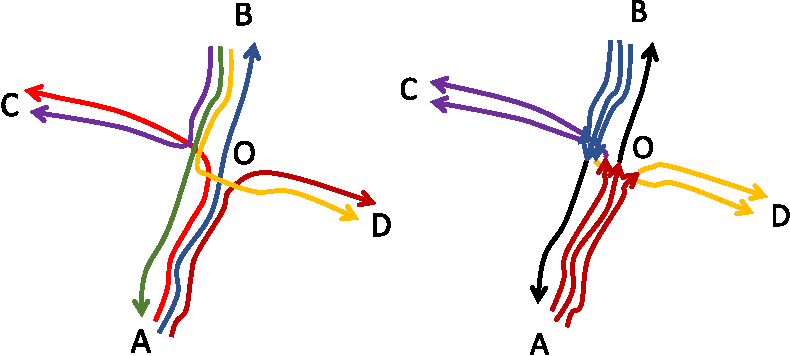
\includegraphics[scale=.8]{res/fig/sec-1/DSCDataset.pdf}
  \caption{Traiettorie di partenza (a sinistra), Cluster individuati da DSC (a destra), Fonte:~\cite{tampakis2019scalable} }%
  \label{fig:chap-1:dsc}
\end{figure}    


Il clustering sovrapposto permette di conservare le relazioni intra-cluster, tuttavia una frammentazione troppo fine può causare
la perdita di \textit{rare pattern}, ad esempio eventi significanti che accadono con una bassa frequenza~\cite{DBLP:journals/tkdd/KohR16, DBLP:journals/geoinformatica/HuangPX06}.

\subsection{Applicazioni e limiti}\label{subsec:problem:applicationandlimits}
Nelle sezioni precedenti sono state prese in considerazione le principali categorie di clustering di dati di traiettoria; queste sono state impiegate in
diversi ambiti, a seconda delle singole caratteristiche della tecnica utilizzata.

Di seguito sono riportati i principali ambiti applicativi del clustering di traiettorie:

\begin{itemize}

  \item \textbf{Analisi dei pattern di movimento degli oggetti.}
  L'applicazione più scontata di un raggruppamento di traiettorie: l'analisi di pattern di
  movimento mira ad individuare quali oggetti si sono mossi assieme secondo certe regole.

  \item \textbf{Previsione dei movimenti di un oggetto.}
  Sulla base delle caratteristiche di una traiettoria, è possibile predirre quali saranno
  i futuri movimenti di un oggetto partendo dai suoi spostamenti passati: si attribuisce infatti
  il percorso fin d'ora eseguito a uno dei cluster individuati e considerando le sue proprietà
  si può predirre con una certa accuratezza il percorso futuro dell'oggetto.
  La validità di questa previsione è direttamente collegata al numero di misure considerate durante
  le operazioni di clustering: maggiore il numero, più accurato il risultato.
  Importanza particolare ha il tempo: non considerandolo è di fatto impossibile eseguire questo tipo
  di ricerca.

  \item \textbf{Supporto alla pianificazione stradale e dei trasporti.}
  Come affermato nella~\cref*{subsec:problem:spatialalgorithms}, determinati algoritmi
  possono individuare i punti più frequentati da certi utenti; è quindi possibile integrare queste
  informazioni in piani di controllo del traffico/ espansione delle infrastrutture urbane.

  \item \textbf{Ricerca di Outlier.}
  Un outlier è per definizione un elemento che, dato un certo criterio di similarità,
  si discosta da tutti gli altri. Gli outlier possono essere interpretati come errori, ma anche
  come comportamenti che per determinati motivi divergono dalla norma.
  Sotto quest'ultima chiave di lettura divengono interessanti la loro ricerca e i motivi per cui
  differiscono dagli altri dati nel dataset.
  Essendo poi il percoso di un oggetto interpretabile come l'insieme dei suoi comportamenti,
  gli outlier individuano comportamenti inusuali e per questo possono destare grande interesse.

  \item \textbf{De-Anonimizzazione dei dati.}
  Utilizzando tecniche di clustering su dati incerti, è possibile ricavare informazioni sugli
  oggetti collegati alle traiettorie precedentemente nascosti tramite tecniche di anonimizzazione.

\end{itemize}

Gli ambiti di utilizzo del clustering di traiettorie sono numerosi, tuttavia il margine di miglioramento
è ancora abbondante.
In primo luogo la maggior parte degli algoritmi non sfrutta tutto il potenziale semantico dei dati:
molte tecniche impiegano solo le dimensioni spazio-temporali o un insieme ristretto di feature,
scartando così informazioni che potrebbero ulteriormente migliorare la qualità dei risultati.
Successivamente i risultati prodotti sono di difficile intrepretazione, molto spesso accade che
l'estrazione di conoscenza mostri relazioni banali o al contrario troppo complesse per essere spiegate.
Infine manca ancora un'integrazione diffusa con le tecnologie di elaborazione Big Data:
la maggior parte degli algoritmi infatti è pensata per computare in maniera centralizzata, rinunciando
ai vantaggi del calcolo distribuito. In questo modo larghi dataset producono risultati di scarsa
qualità in tempi alti.
L'applicazione di queste strategie di computazione, sebbene complessa nella sua realizzaione, porterebbe
notevoli vantaggi e supererebbe molte delle problematiche degli attuali algoritmi.
I framework \textit{G.C.M.P}\cite{DBLP:journals/pvldb/FanZWT16} e \textit{C.U.T.E} pongono questo
supporto come uno dei loro punti di forza.





\section{Frequent itemset mining}\label{sec:fim}
Nell'ambito dell'analisi dei dati, il \textit{frequent itemset mining}, o ricerca di itemset frequenti,
è uno dei task con maggiori ambiti di applicazione: può essere impiegato nei processi di classificazione,
clustering o ricerca di outlier~\cite{article}.

Il frequent itemset mining necessita di un insieme di transazioni per effettuare la propria ricerca,
ogni transazione, o riga (\textit{row}) che dir si voglia, è composta poi da un insieme di attributi,
o \text{feature}, che identificano gli elementi all'interno della singola transazione.
Occorre specificare che di una feature è considerata rilevante ai fini della ricerca solo la presenza
o l'assenza e non un eventuale valore o altre proprietà collegate; queste potranno essere integrate
mediante apposite tecniche di preprocessing.

Scopo del mining di itemset frequenti è di ricercare, dato un insieme di transazioni, ricercare
le combinazioni di feature, o itemset, che risultano frequenti.
Misura fondamentale per definire la frequenza è il supporto: tale metrica può essere
descritta come il numero di transazioni che contengono un certo itemset.
All'interno della ricerca di itemset frequenti viene definito un limite inferiore al supporto
per determinare l'interesse verso un certo itemset; questo parametro prende il nome
di supporto minimo, o \textit{minsup}.
Definito ciò, è possibile esprimere il problema del mining di itemset frequenti con
la seguente formulazione (~\cref{definition:fim}) :

\begin{definition}[Frequent Itemset Mining]\label{definition:fim}
  Definito \(T\) come l'insieme delle transazioni e \(F\) come quello delle feature complessive,
  il frequent itemset mining ricerca tutti gli itemset \\
  \( i = \{ f_{1}, \ldots, f_{n}\}, f_{1}, \ldots, f_{n} \in F\)
  tali che definito il supporto \( S = \{ t_{1}, \ldots, t_{m} \} \in T \; s.t \; \forall t_{i} \in \{ t_{1}, \ldots, t_{m} \}
  i \subseteq t_{i}  \), \(|S| \geq minsup\)
\end{definition}

Definito l'obbiettivo della ricerca, sono necessari due passaggi per realizzarla:
il primo passo consiste nella generazione di tutti i possibili itemset, il secondo
nel calcolo del supporto per ciascuno di questi e \textit{pruning} (potatura) dei candidati
non interessanti.
Nonostante la definizione semplice, la complessità computazionale di queste fasi può esplodere:
supponendo infatti di avere un set di feature contenente \(n\) diversi elementi, l'insieme di tutte
le possibili combinazioni generabili è \(2^n\), rendendo di fatto molto costoso il processo
di ricerca in presenza di dataset di larghe dimensioni.


\subsection{Algoritmo Apriori}\label{subsec:apriori}
\textit{Apriori}~\cite{agarwal2001tree} è un algoritmo pensato per affrontare il problema della generazione
e filtraggio dei candidati in maniera efficace e efficiente.
Apriori utilizza una struttura di generazione a livelli in maniera iterativa: ad ogni livello sono ricercati pattern di dimensioni \(k\)
aventi supporto maggiore di \(minsupp\).
Successivamente i pattern validi sono impiegati nella costruzione
del livello successivo, mentre gli altri sono scartati.
Intuitivamente, la ragione per cui accade ciò è che la frequenza di un set sarà sempre maggiore di
quella di qualunque superset a cui questo appartiene.Se già un set non soddisfa il vincolo di frequenza,
nessun suo superset potrà fare altrettanto.
Ne segue che tutti gli itemset generati al livello \(k + 1\) saranno combinazioni di pattern validi al livello
\(k\).
Questa strategia di generazione permette di scartare un grande numero di itemset e le loro successive
combinazioni (~\cref{fig:chap-1:apriori-example}).

\begin{figure}
  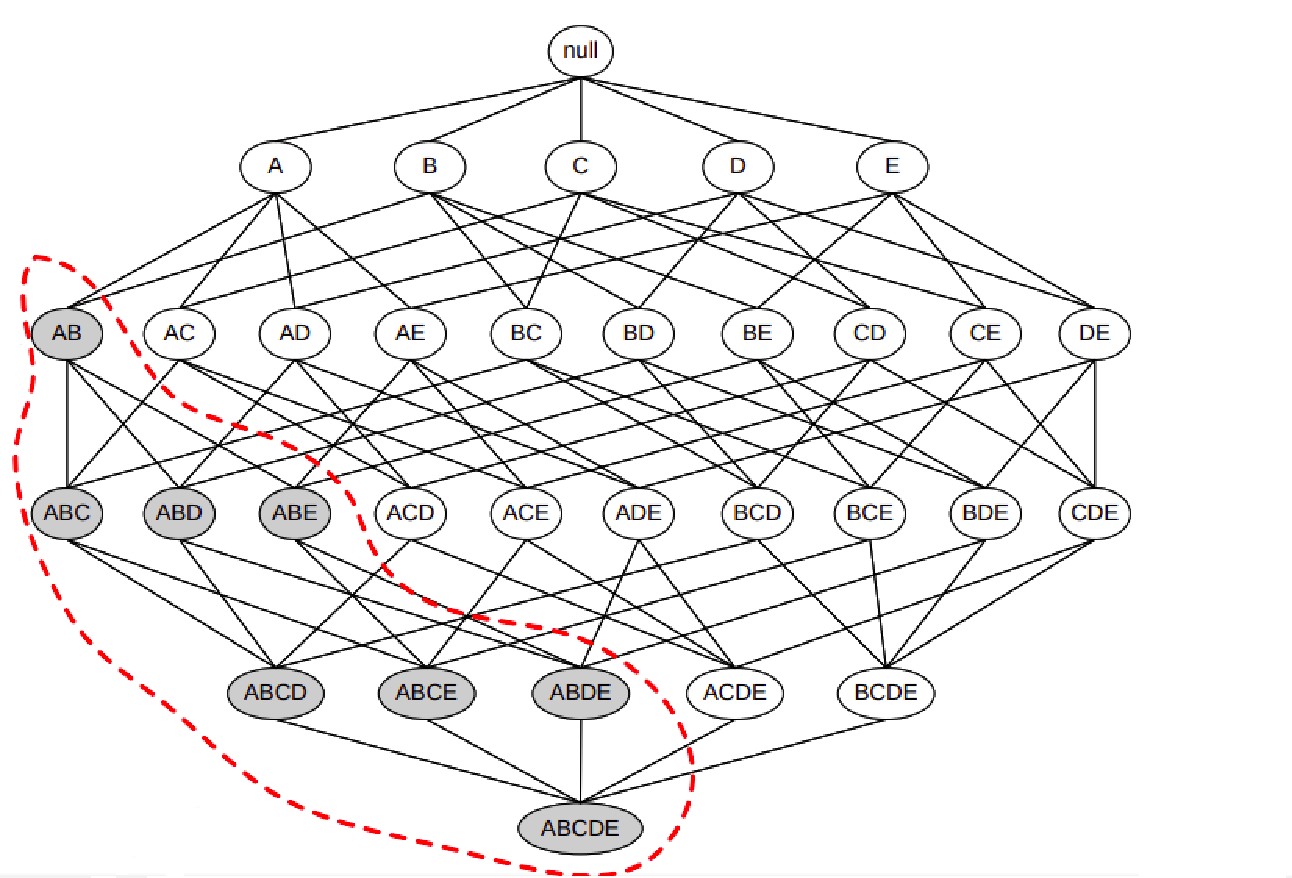
\includegraphics[scale=.8]{/sec-1/APrioriExample.pdf}
  \caption{Esempio di struttura gerarchica generata dall'algoritmo Apriori, in questo caso l'itemset \( \{ a,b \} \) non risulta frequente, di conseguenza i suoi superset sono scartati,Fonte:~\url{http://bias.csr.unibo.it/golfarelli/DataMining/MaterialeDidattico/2017/11-RegoleAssociative.pdf}}%
  \label{fig:chap-1:apriori-example}
\end{figure}

All'interno dell'insieme degli itemset validi, è possibile eseguire un'ulteriore distinzione:
si definiscono chiusi (\textit{closed}) gli itemset aventi supporto strettamente maggiore di
tutti i propri superset; al contrario un itemset non avente superset validi è definibile come
massimale (\textit{maximal}).

In molti casi Apriori è efficace nel ridurre lo spazio di ricerca di itemset validi, tuttavia
soffre di alcuni limiti: in primo luogo è molto probabile che il numero di candidati generati rimanga comunque
alto, in quanto molti di questi sono generati in un primo momento e scartati dopo il calcolo del supporto.
Proprio a quest'ultimo punto si collega un'altra problematica: la computazione del supporto richiede molte
scansioni delle transazioni e ad ogni livello devono essere verificati molti itemset.


\subsection{Frequent itemset mining su dati di traiettoria}\label{subsec:fim-trajectory}
La ricerca di itemset frequenti può essere adattata ai dati di traiettoria.
Ciò non è altro che un'evoluzione del mining di sequenze.

Il mining di pattern su un insieme di item è un caso particolare di mining di itemset frequenti.
La principale modifica è l'introduzione del concetto di tempo e , conseguentemente, di sequenza.
Una sequenza non è altro che un itemset i cui elementi sono ordinati rispetto al tempo.
Ad esempio, l'itemset \(<a, ab, c>\) può essere interpretato come una sequenza in cui i tre elementi
si susseguono in istanti temporali contigui.
Nella ricerca di sequenze, gli attributi sono espliciti.
Nel caso dei dati di traiettoria però, ciò non risulta vero: ogni punto di traiettoria grezza è composto da latitudine, longitudine e istante temporale.
Tali punti sono difficilmente coincidenti tra loro, ciò causa una difficoltà nell'estrazione delle feature.
Per superare questa problematica, occorre ricorrere all'utilizzo di astrazioni di traiettoria:
mappando il dataset su uno specifico sistema di riferimento, è possibile accomunare i punti negli stessi quanti.

Questa astrazione consente di superare certi limiti, tuttavia non è sufficiente a risolvere il problema.
Gli algoritmi di riconoscimento di itemset frequenti o sequenze, oltre ad avere un alto costo computazionale, non sono in grado di processare la contiguità spaziale e la continuità temporale.
Inoltre nel riconoscimento di sequenze sono richieste strette relazioni di adiacenza tra le feature, cosa non sempre possibile nelle traiettoria, a causa della loro intrinseca incertezza.

In letteratura sono state proposte diverse soluzioni per superare questi limiti:
ad esempio per quanto riguarda la generazione delle sequenze è stato proposto l'utilizzo di una struttura ad albero per generare i pattern di movimento \cite{cao2005mining}.
Per quanto riguarda invece le relazioni ignorate, sono stati proposti approcci per considerare la contiguità spaziale \cite{chen2011personal} e quella temporale \cite{lv2015route}. 

Le applicazioni del mining di traiettorie presenti in letteratura riguardano l'estrazione dei percorsi 
più frequentati \cite{qiu2016mining} e delle regioni più trafficate \cite{zheng2018spatial}.
È interessante considerare come la ricerca di luoghi e percorsi frequentati sia ortogonale rispetto all'individuazione di gruppi di oggetti che hanno viaggiato assieme per un certo periodo di tempo.
Approfondendo questo confronto, emerge che la definizione del problema è molto simile, ma cambia il ruolo di transazioni e feature.
Nel caso di ricerca di luoghi frequenti in un dataset, tale frequenza è determinata sulla base degli oggetti che passano per un certo punto.
Trattando invece di analisi di oggetti che si sono mossi assieme, 
intuitivamente il supporto è definibile come l'insieme di posizioni condivise dal gruppo perché sia considerato frequente.

La ricerca di gruppi di oggetti non è affrontabile con le ordinarie tecniche di itemset mining.
Il numero degli oggetti infatti supera di gran lunga quello delle posizioni visitate, di conseguenza 
l'insieme delle transazioni avrebbe cardinalità molto inferiore rispetto a quello delle feature.
Tale condizione esplode il costo computazionale per la ricerca di itemset frequenti.


